\documentclass[default]{beamer}
\usetheme{default} % https://hartwork.org/beamer-theme-matrix/
\usepackage{beamerthemetree} 
\usepackage{hyperref}
\hypersetup{
  colorlinks=true,
  urlcolor=blue
}
\beamertemplatenavigationsymbolsempty

\title{KubeCon '19 Barcelona}
\author{Daniel-Andrei Minca}
\institute{Site Reliability Engineer @ GfK SE}
\date{20-23 May '19}

\begin{document}

\begin{frame}
  \titlepage
\end{frame}
\note{Talk for 15 minutes}

\section[Outline]{Outline}
\begin{frame}
  \frametitle{Outline}
  \begin{enumerate}
    \note{3min / item + 6 min demo}
    \item D1 - Intro
    \item D2 - Deep-dive
    \item D3 - Wrap-up
    \item Demo: 'kind' (Kubernetes in Docker)\footnotemark
  \end{enumerate}
  \footnotetext[1]{pray to the demo gods}
\end{frame}

\note{At the end, make a Demo on 'kind' - Kubernetes in Docker}

\section{Day 0 - bonus}
\begin{frame}
  \frametitle{Beer?}
  \begin{figure}
    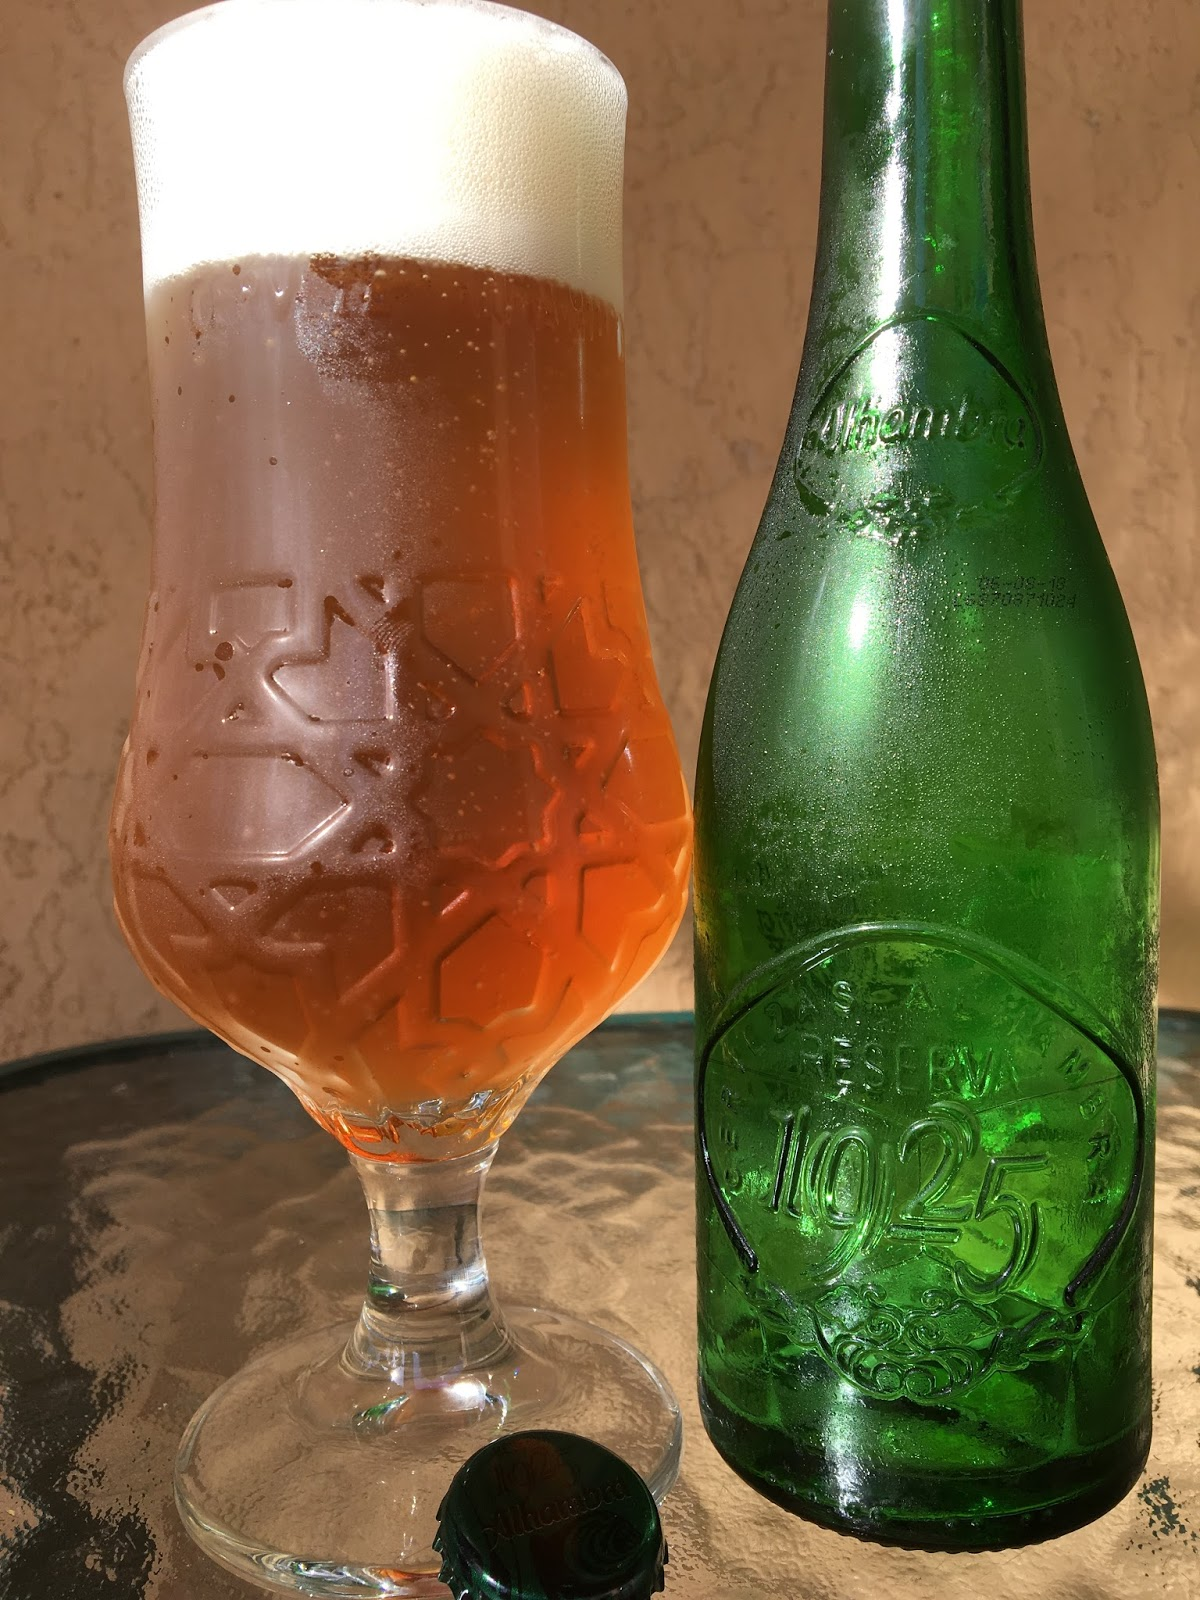
\includegraphics[width=110pt,height=160pt]{src/kubecon/static/beer.jpg}
    \caption{Alhambra - mana potion}
  \end{figure}
\end{frame}

\section{Day 1 - intro}


\begin{frame}
  \frametitle{State of CNCF projects}\footnotemark
  \note{Istio we have a problem - Understanding and fixing bugs in a Service Mesh, David Gageot (Google)}
  \begin{enumerate}
    \item Incubating:
    \begin{itemize}
      \item Linkerd
      \item Helm v3.0.0-alpha1 w/o Tiller
      \item Rook.io
      \item Harbor etc.
    \end{itemize}
    \item Graduated:
    \begin{itemize}
      \item fluentd
    \end{itemize}
  \end{enumerate}
  \footnotetext[2]{https://youtu.be/vdxcaR3I2ic?t=728}
\end{frame}

\begin{frame}
  \frametitle{Top players at KubeCon '19}   % Insert frame title between curly braces
  \begin{columns}[c]
    \column{2in}
      \begin{itemize}
        \item Google Cloud Platform
        \item Amazon Web Services
        \item WeaveWorks
      \end{itemize}
    \column{2in}
    \begin{figure}
      
\includegraphics[width=90pt,height=150pt]{src/kubecon/static/img01.jpeg}
      \caption{Huawei was also there}
    \end{figure}
  \end{columns}
\end{frame}


\section{Day 2 - deep-dives}


\subsection{Loki}
\begin{frame}
  \frametitle{Loki (by Grafana)\footnotemark}
  \begin{columns}
    \column{2in}
    \begin{itemize}
      \item logs: groups them into 'streams' \& indexes them with labels
      \item LogQL allows filter chaining
      \item extract labels from logs
      \item live tailing (demo failed during KubeCon pres.)
    \end{itemize}
    \column{2in}
    \begin{figure}
      
\includegraphics[width=150pt,height=80pt]{src/kubecon/static/loki.png}
    \end{figure}
  \end{columns}
  \footnotetext[3]{\href{https://youtu.be/CQiawXlgabQ}{https://youtu.be/CQiawXlgabQ}}
\end{frame}

\subsection{Linkerd}
\begin{frame}
  \frametitle{Linkerd\footnotemark}
  \begin{columns}
    \column{2in}
    \begin{enumerate}
      \item service mesh: sidecar, data-plane etc.
      \item auto golden-metrics
      \item transparent mTLS
    \end{enumerate}
    \column{2in}
    \begin{figure}
      
\includegraphics[width=150pt,height=40pt]{src/kubecon/static/linkerd.png}
    \end{figure}
  \end{columns}
  \footnotetext[4]{\href{https://youtu.be/Z3nfLI3z0hc}{https://youtu.be/Z3nfLI3z0hc}}
\end{frame}

\subsection{Kubernetes Dashboard (Grafana)}
\begin{frame}
  \frametitle{Kubernetes Dashboard (by Grafana)\footnotemark}
  \begin{enumerate}
    \item DMM (Dashboard Maturity Model)
    \item template variables (use more)
    \item Use scripting libraries to \href{https://www.youtube.com/watch?v=GDdnL5R_l-Y}{generate dashboards (mixins)}
    \begin{itemize}
      \item \href{https://github.com/grafana/grafonnet-lib}{grafonnet (Jsonnet)}
      \item \href{https://github.com/weaveworks/grafanalib}{grafanalib (Python)}
    \end{itemize}
  \end{enumerate}
  \footnotetext[4]{\href{https://youtu.be/YE2aQFiMGfY}{https://youtu.be/YE2aQFiMGfY}}
\end{frame}


\section{Day 3 - wrap-up}


\subsection{Istio}
\begin{frame}
  \frametitle{Istio\footnotemark}
  \begin{figure}
    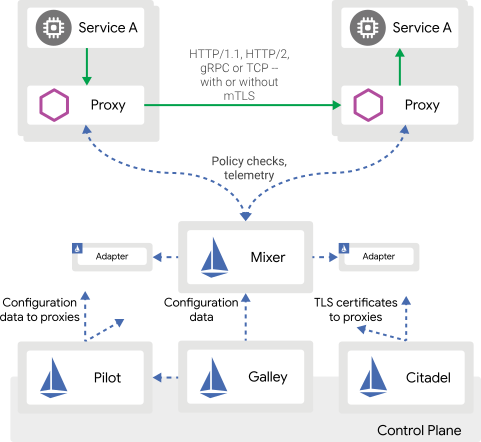
\includegraphics[width=200pt,height=150pt]{src/kubecon/static/istio2.png}
  \end{figure}
  \begin{enumerate}
    \item Grants: mTLS, ACL, traffic auditing, passthrough mTLS, auto LB
    \item Conn's multiple net's through Gateways
  \end{enumerate}
  \footnotetext[5]{\href{https://youtu.be/-t2BfT59zJA}{https://youtu.be/-t2BfT59zJA}}
\end{frame}

\begin{frame}
  \begin{figure}
    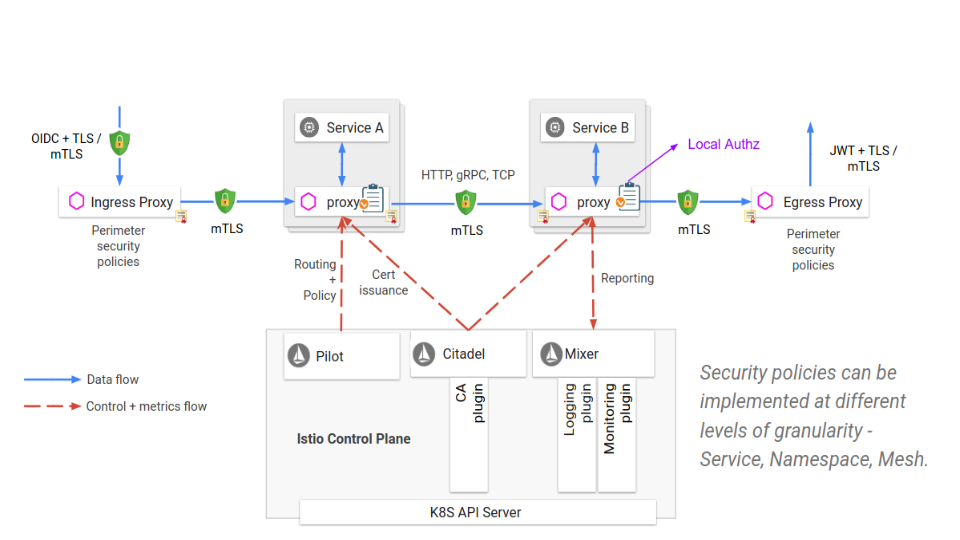
\includegraphics[width=300pt,height=150pt]{src/kubecon/static/istio.png}
    \caption{Istio mTLS (security)}
  \end{figure}
\end{frame}
% \subsection{Envoy}
% \begin{frame}
%   \frametitle{Envoy\footnotemark}
%   \begin{enumerate}
%     \item Layer 7 proxy
%     \item HTTP/2 support
%     \item New: Kafka support
%     \item gRPC, HTTP L7 routing etc.
%   \end{enumerate}
%   \footnotetext[5]{\href{https://www.envoyproxy.io/docs/envoy/latest/intro/what\_is\_envoy}{envoy docs because the presentation sucked}}
% \end{frame}

\subsection{CI/CD - 'kind'}
\begin{frame}
  \frametitle{CI/CD with 'kind'\footnotemark}
  \begin{columns}
    \column{2in}
    \begin{enumerate}
      \item e2e tests:
      \begin{itemize}
        \item start full k8s Cluster
        \item black-box Testing
        \item 'kind create cluster'
      \end{itemize}
      \item exposes full kubeadm config surface
      \item enable Alpha features, Network Driver etc.
    \end{enumerate}
    \column{2in}
    \begin{figure}
      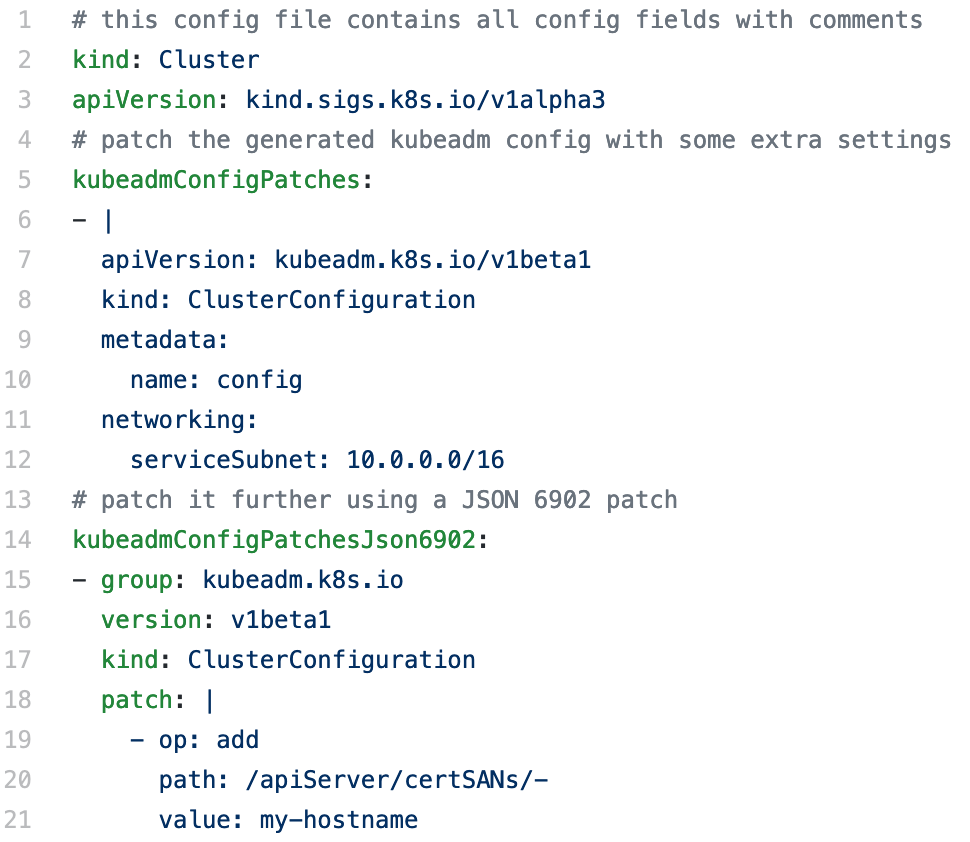
\includegraphics[width=130pt,height=100pt]{src/kubecon/static/kind.png}
      \caption{sample \href{https://github.com/kubernetes-sigs/kind/blob/master/site/content/docs/user/kind-example-config.yaml}{'kind' config file}}
    \end{figure}
  \end{columns}
  \footnotetext[3]{\href{https://youtu.be/8KtmevMFfxA}{https://youtu.be/8KtmevMFfxA}}
\end{frame}

\begin{frame}
  \begin{columns}
    \column{2in}
    \begin{enumerate}
      \item \href{https://github.com/kind-ci/examples}{examples of kind running on XYZ CI}
      \item other ways to run kind:
      \begin{itemize}
        \item as a library
      \end{itemize}
    \end{enumerate}
    \column{2in}
    \begin{figure}
      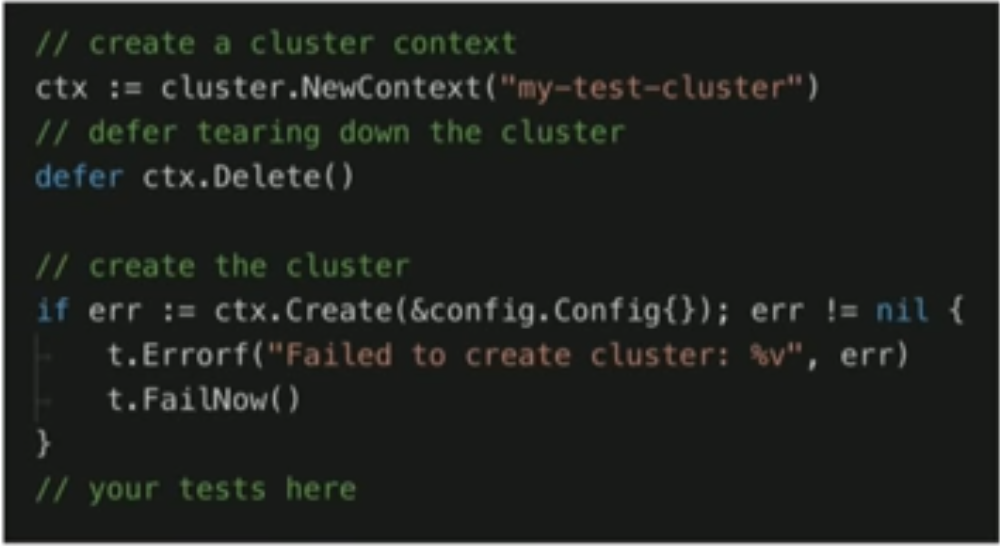
\includegraphics[width=190pt,height=100pt]{src/kubecon/static/kind2.png}
    \end{figure}
  \end{columns}
\end{frame}

\section{Demo time!}


\begin{frame}
  \frametitle{DEMO: kind}
  \begin{figure}
    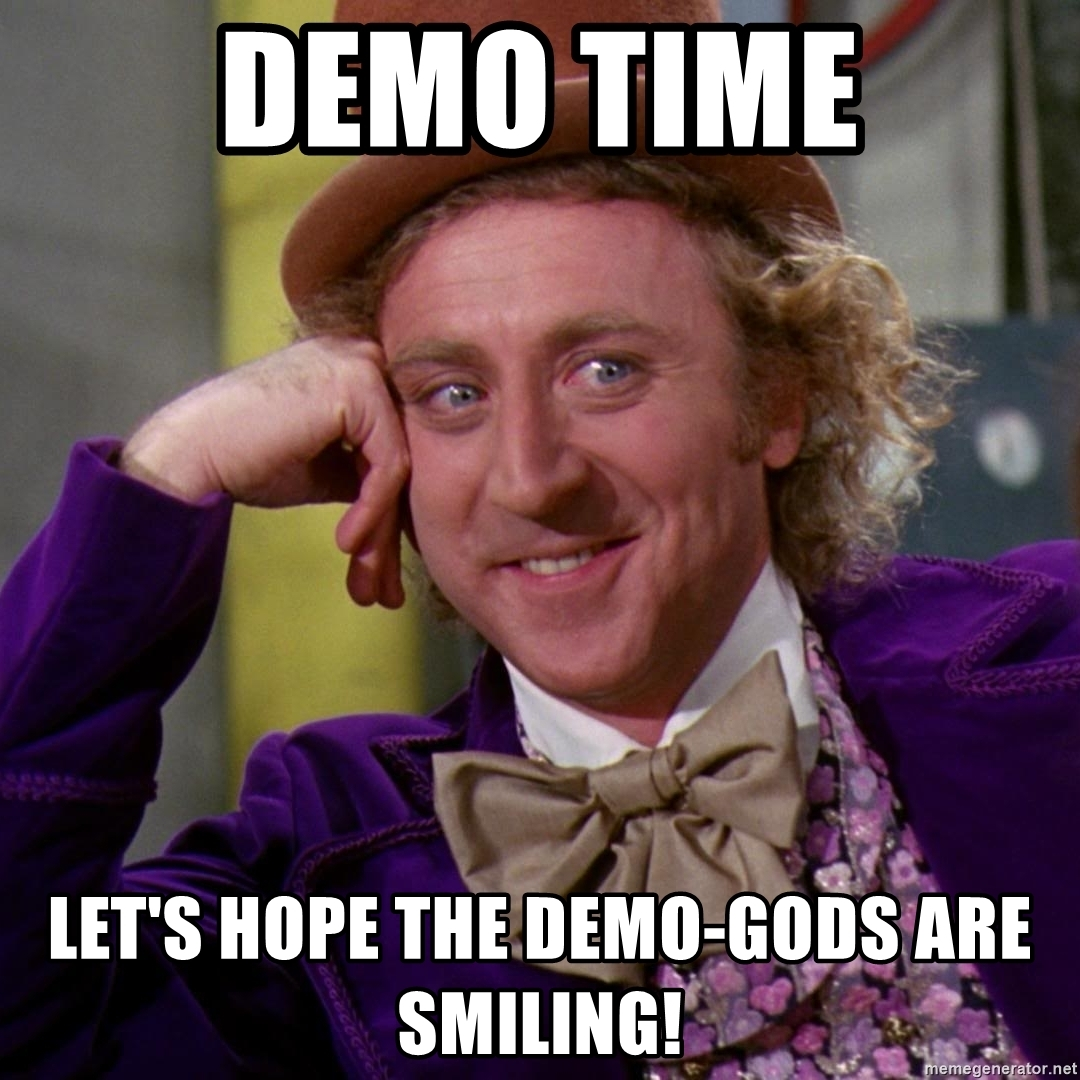
\includegraphics[width=150pt,height=150pt]{src/kubecon/static/demo.jpg}
  \end{figure}
\end{frame}

\section{Refs}
\begin{frame}
  \frametitle{Refs \& links}
  \begin{itemize}
    \item \url{https://static.sched.com/hosted_files/kccnceu19/31/Grafana\%20Loki.pdf}
    \item \url{https://static.sched.com/hosted_files/kccnceu19/e8/Intro\%20to\%20Linkerd\%20KCCNCEU19.pdf}
    \item \url{https://static.sched.com/hosted_files/kccnceu19/27/Kubecon\%202019_\%20Kubernetes\%20dashboards\%20final.pdf}
    \item \url{https://www.youtube.com/playlist?list=PLj6h78yzYM2PpmMAnvpvsnR4c27wJePh3}
  \end{itemize}
\end{frame}
\end{document}
